
\documentclass{exam}

\usepackage{units} 
\usepackage{siunitx} 
\usepackage{graphicx}
\usepackage[fleqn]{amsmath}
\usepackage{cancel}
\usepackage{float}
\usepackage{mdwlist}
\usepackage{booktabs}
\usepackage{cancel}
\usepackage{polynom}
\usepackage{caption}
\usepackage{fullpage}
\usepackage{xfrac}
\usepackage{enumerate}
\usepackage{comment}

\newcommand{\degree}{\ensuremath{^\circ}} 
\everymath{\displaystyle}

% \begin{figure}[H]
%   \centering
%   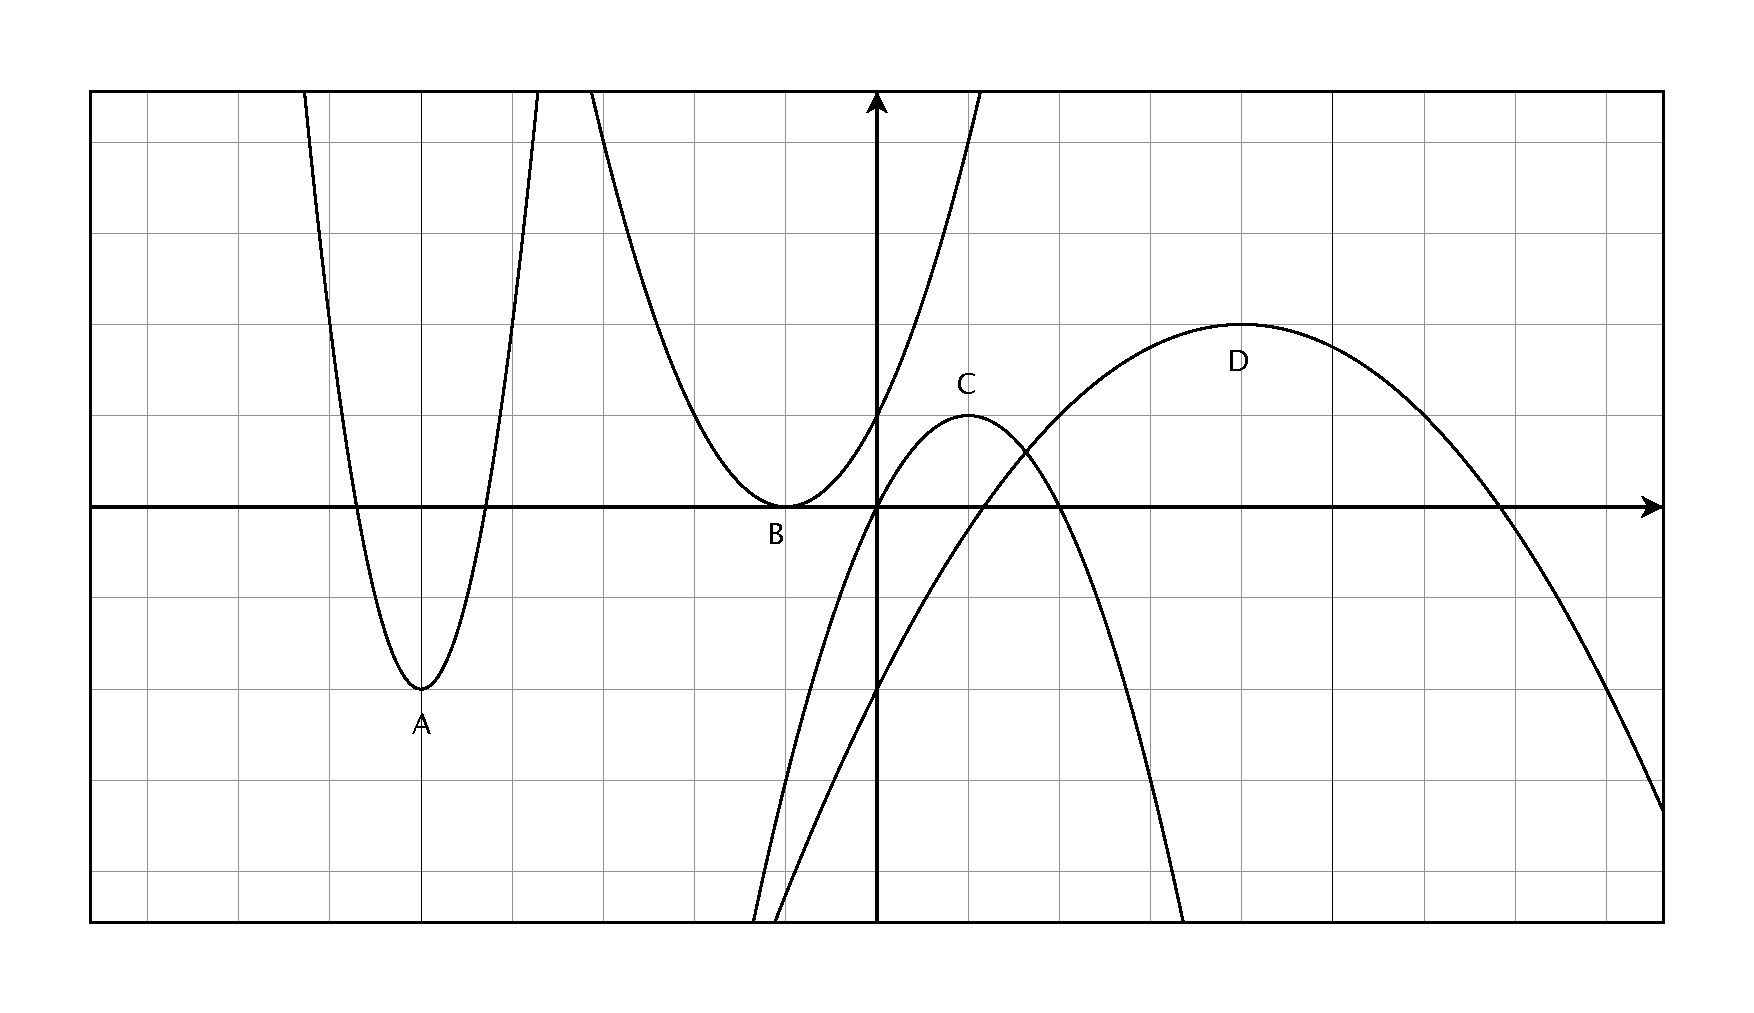
\includegraphics[scale=.3]{problem_7.eps}
%   \caption*{Problem 7}
% \end{figure}

% \begin{tabular}{cc}
% \toprule
% period & amplitude \\
% \midrule
%   $\pi$ & $2$ \\
% \bottomrule
% \end{tabular}

\printanswers

\ifprintanswers 
  \usepackage{2in1, lscape} 
\fi

\date{January 30, 2013}
\title{Math 141 \\ Homework 4}

\begin{document}

\excludecomment{comment}

\maketitle

\section{Homework}

\begin{itemize*}
  \item Read Section 2.5 and 2.6
  \item Section 2.5: 1-2, 6-10, 17, 20-21, 27, 29-30, 35, 38-41, 45-46, 47-48, 59-61
  \item Section 2.6: 1-5, 12-13, 17, 20, 23
\end{itemize*}

\section{Extra Credit}
Section 2.6, problem 29

\ifprintanswers
  \pagebreak
  \begin{solution}
    \begin{parts}
      \part
        The perimeter contains half of a circle, the bottom of the rectangle, and the two sides:
        \[
          P = \frac{\pi x}{2} + x + 2h
        \]
        Solve for $h$:
        \[
          h = \frac{P}{2} - \frac{x}{2} - \frac{\pi x}{4}
        \]

        The area contains half of a circle and a rectangle:
        \[
          A = \frac{1}{2} \pi \left( \frac{x}{2} \right)^2 + xh = \frac{\pi x^2}{8} + xh
        \]

        Substitute the expression for $h$ in the area equation:
        \begin{align*}
          A &= \frac{\pi x^2}{8} + x \left( \frac{P}{2} - \frac{x}{2} - \frac{\pi x}{4} \right) \\
            &= \frac{P}{2} x - x^2 \left( \frac{\pi + 4}{8} \right) \\
        \end{align*}

        For this problem, the perimeter is 30 ft, so the final function is:
        \[
          A(x) = 15x - x^2 \left( \frac{\pi + 4}{8} \right) \\
        \]
      
        \part
          Convert the fractions to decimals and find the maximum:
          \begin{align*}
            A(x)    &= -0.8927x^2 + 15x \\
            x_{max} &= \frac{-15}{2 \left( -0.8927 \right) } \\
                    &= 8.401 \\
          \end{align*}

          The largest area of approximately $\SI{63.011}{ft^2}$ is achieved when $x \approx \SI{8.401}{ft}$.
    \end{parts}
  \end{solution}

  \pagebreak

  \section{Section 2.5}

  \begin{description}
    \item[1] 
      \begin{parts}
        \part vertex: $(3, 4)$
        \part the maximum value of 4 occurs when $x = 3$
      \end{parts}

    \item[2] 
      \begin{parts}
        \part vertex: $(-2, 8)$
        \part the maximum value of $8$ occurs when $x = -2$
      \end{parts}

%    \item[5]
%      Put in standard form to find the vertex:
%      \begin{align*}
%        f(x) &= x^2 - 6x \\
%          &= x^2 - 6x + 9 - 9 \\
%          &= (x - 3)^2 - 9 \\
%      \end{align*}
%      The vertex is at $(3, -9)$.
%
%      Set to 0 and solve for x to find the x-intercepts:
%      \begin{align*}
%        x^2 - 6x &= 0 \\
%        x(x - 6) &= 0 \\
%        x &= \left\{ 0, 6 \right\} \\
%      \end{align*}
%      The x-intercepts are at $(0, 0)$ and $(6, 0)$.  Since $(0, 0)$ is one of these points, this is also the y-intercept.
%
%      \begin{figure}[H]
%        \centering
%        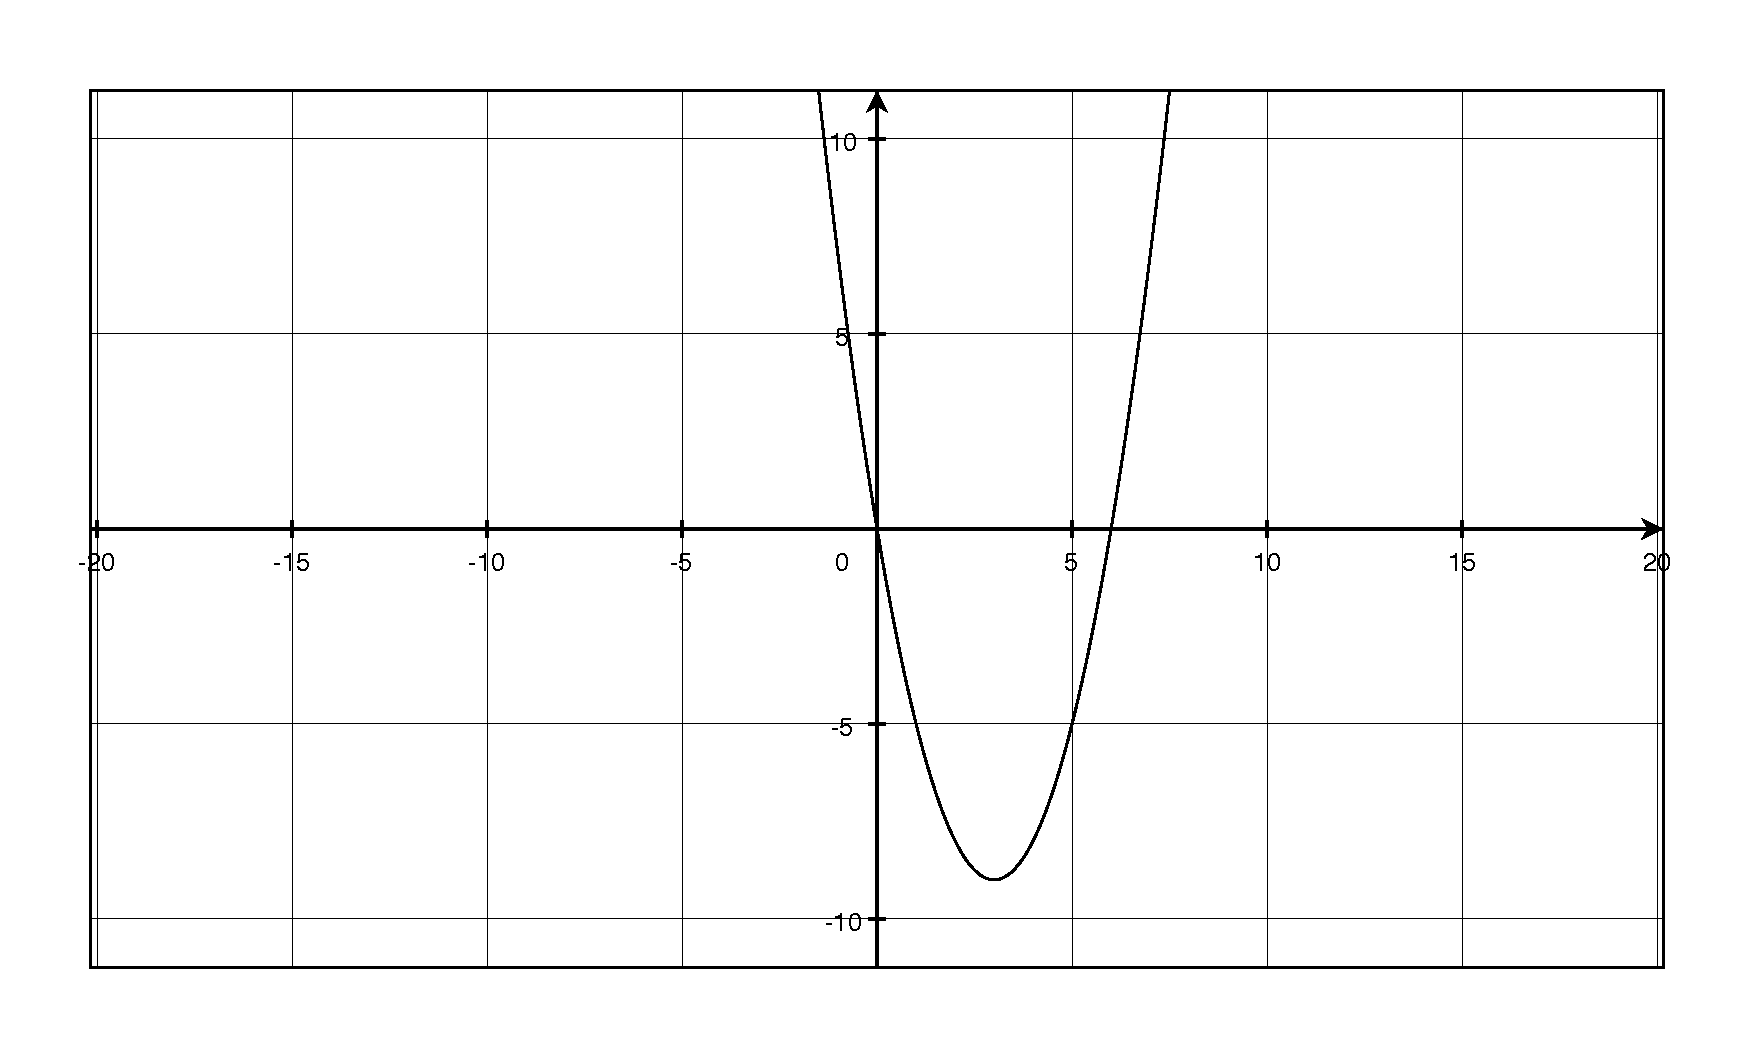
\includegraphics[scale=.3]{problem_05.eps}
%        \caption*{Problem 5}
%      \end{figure}

    \item[6]
      Put in standard form to find the vertex:
      \begin{align*}
        f(x) &= x^2 + 8x \\
             &= x^2 + 8x + 16 - 16 \\
             &= (x + 4)^2 - 16 \\
      \end{align*}
      The vertex is at $(-4, -16)$.

      Set to 0 and solve for x to find the x-intercepts:
      \begin{align*}
        x^2 + 8x &= 0 \\
        x(x + 8) &= 0 \\
        x        &= \left\{ 0, -8 \right\} \\
      \end{align*}
      The x-intercepts are at $(0, 0)$ and $(-8, 0)$.  Since $(0, 0)$ is one of these points, this is also the y-intercept.

      \begin{figure}[H]
        \centering
        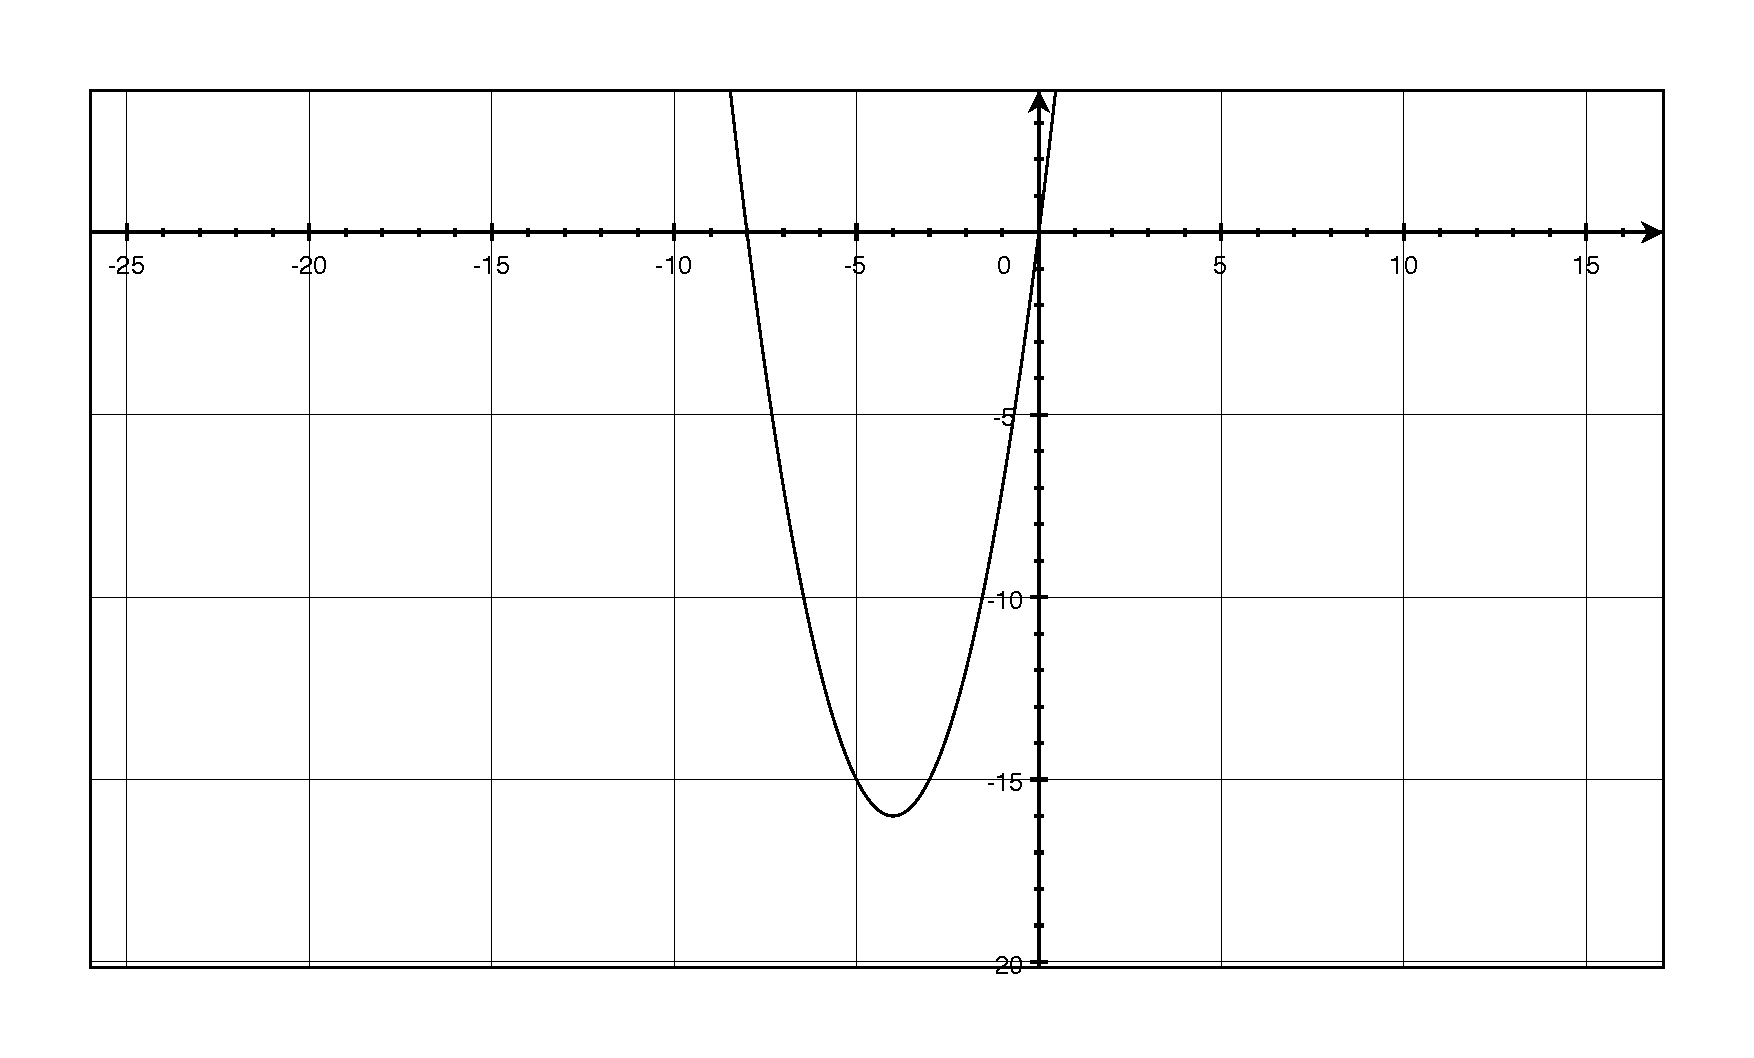
\includegraphics[scale=.3]{problem_06.eps}
        \caption*{Problem 6}
      \end{figure}

    \item[7]
      Put in standard form to find the vertex:
      \begin{align*}
        f(x) &= 2x^2 + 6x \\
             &= 2(x^2 + 3x) \\
             &= 2 \left( x^2 + 3x + \frac{9}{4} - \frac{9}{4} \right) \\
             &= 2 \left( x^2 + 3x + \frac{9}{4} \right) - \frac{9}{2} \\
             &= 2 \left( x + \frac{3}{2} \right)^2 - \frac{9}{2} \\
      \end{align*}
      The vertex is at $\left( -\frac{3}{2}, -\frac{9}{2} \right)$.

      Set to 0 and solve for x to find the x-intercepts:
      \begin{align*}
        2x^2 + 6x &= 0 \\
        x^2 + 3x  &= 0 \\
        x(x + 3)  &= 0 \\
        x         &= \left\{ -3, 0 \right\} \\
      \end{align*}
      The x-intercepts are at $(0, 0)$ and $(-3, 0)$.  Since $(0, 0)$ is one of these points, this is also the y-intercept.

      \begin{figure}[H]
        \centering
        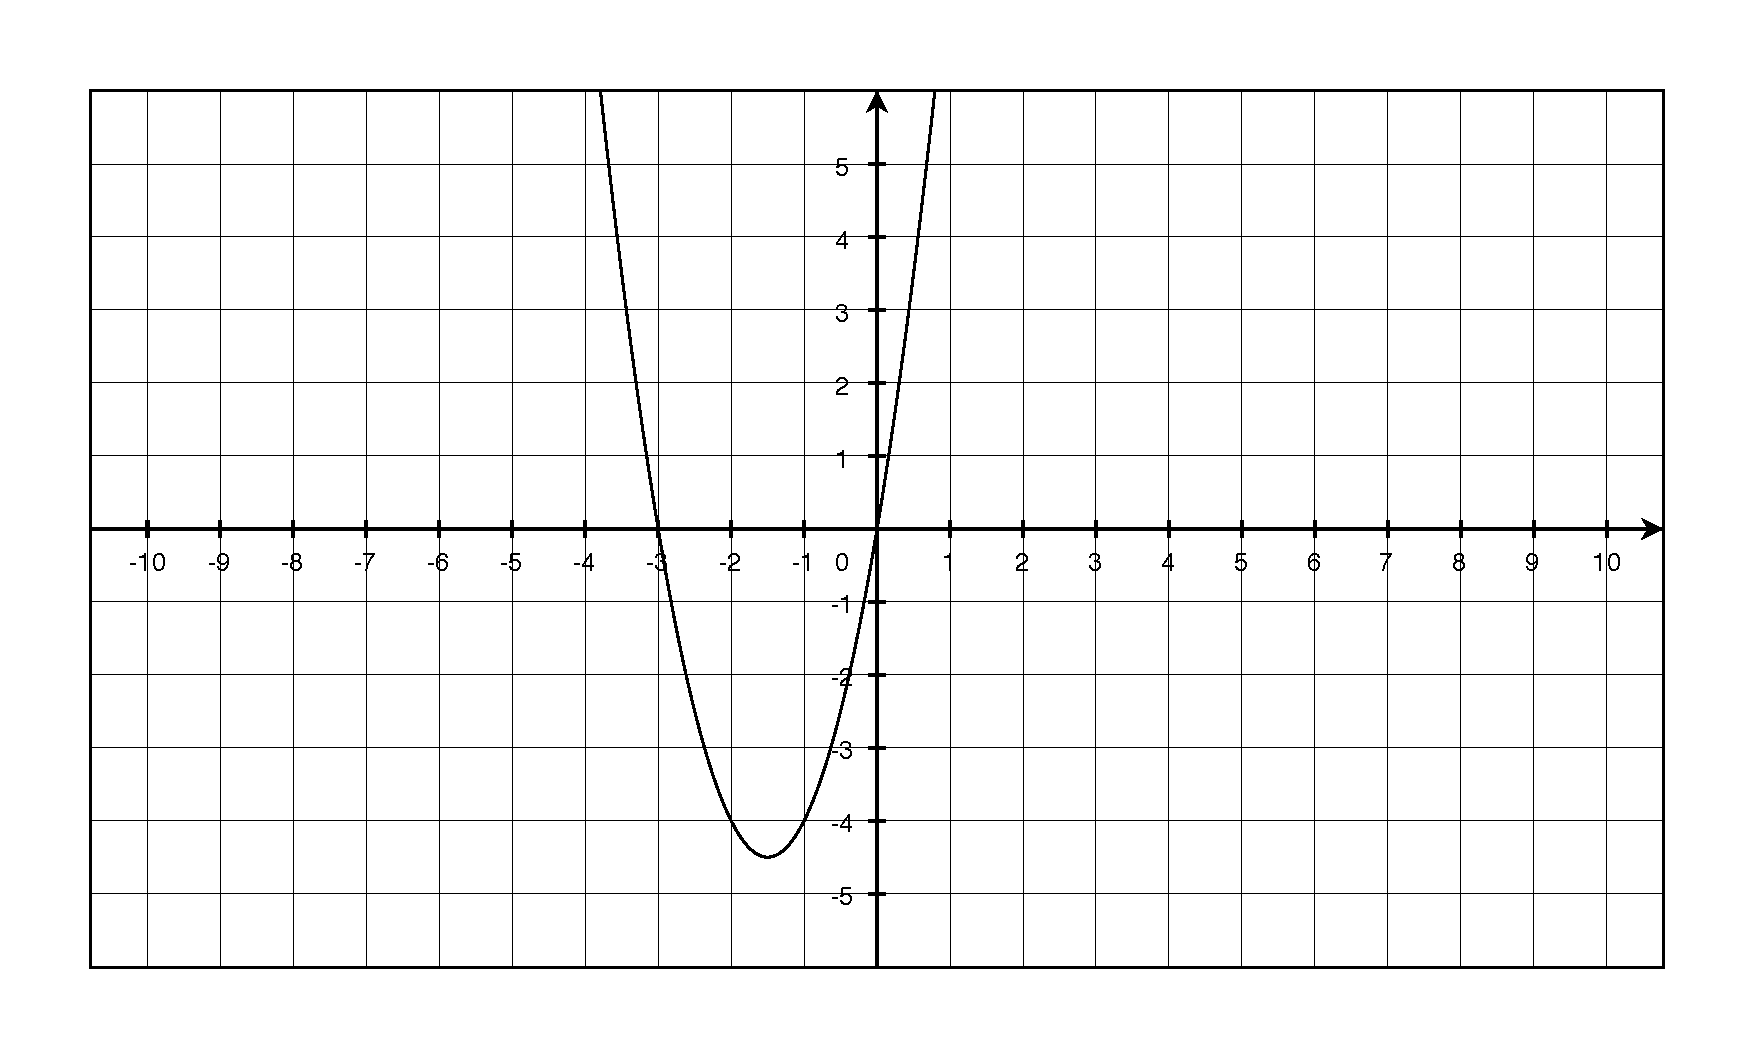
\includegraphics[scale=.3]{problem_07.eps}
        \caption*{Problem 7}
      \end{figure}

    \item[8]
      Put in standard form to find the vertex:
      \begin{align*}
        f(x) &= -x^2 + 10x \\
             &= -(x^2 - 10x) \\
             &= -(x^2 - 10x + 25 - 25) \\
             &= -( (x - 5)^2 - 25) \\
             &= -(x - 5)^2 + 25 \\
      \end{align*}
      The vertex is at $(5, 25)$.

      Set to 0 and solve for x to find the x-intercepts:
      \begin{align*}
        -x^2 + 10x &= 0 \\
        x^2 - 10x  &= 0 \\
        x(x - 10)  &= 0 \\
        x          &= \left\{ 0, 10 \right\} \\
      \end{align*}
      The x-intercepts are at $(0, 0)$ and $(10, 0)$.  Since $(0, 0)$ is one of these points, this is also the y-intercept.

      \begin{figure}[H]
        \centering
        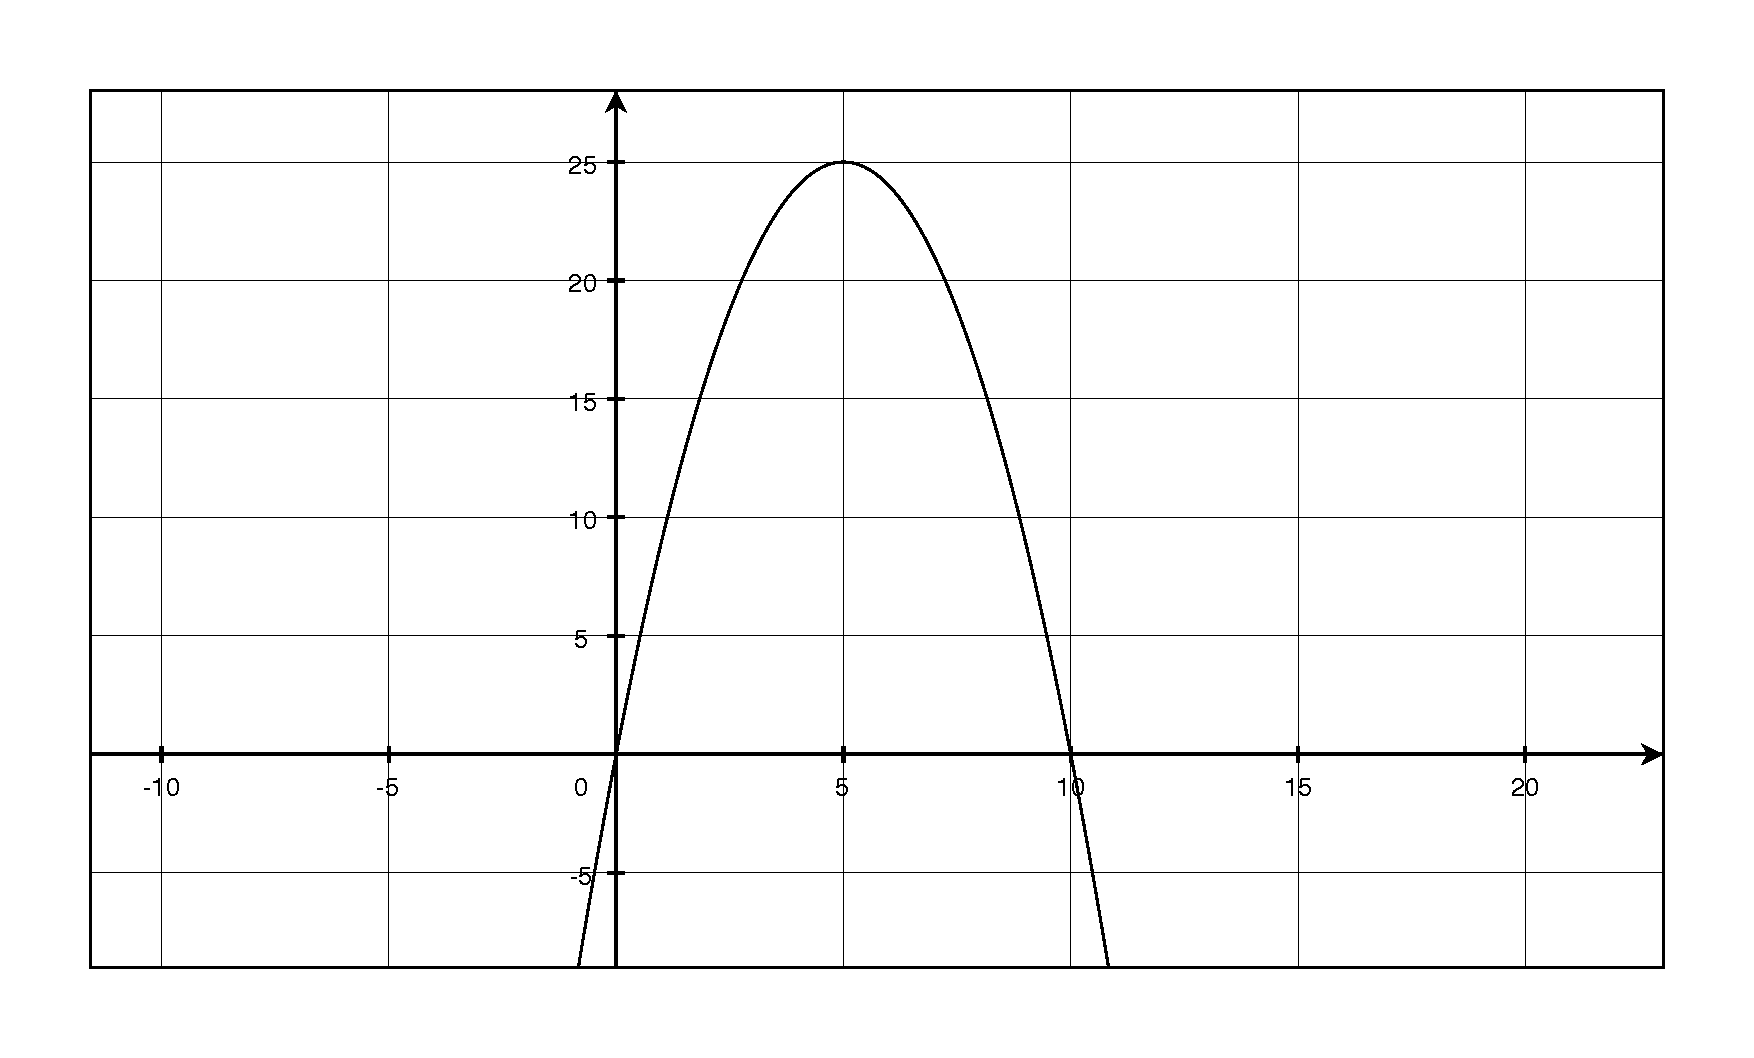
\includegraphics[scale=.3]{problem_08.eps}
        \caption*{Problem 8}
      \end{figure}

    \item[9]
      Put in standard form to find the vertex:
      \begin{align*}
        f(x) &= x^2 + 4x + 3 \\
             &= x^2 + 4x + 4 - 4 + 3 \\
             &= (x + 2)^2 - 1 \\
      \end{align*}
      The vertex is at $(-2, -1)$.

      Set to 0 and solve for x to find the x-intercepts:
      \begin{align*}
        x^2 + 4x + 3   &= 0 \\
        (x + 3)(x + 1) &= 0 \\
        x              &= \left\{ -1, -3 \right\} \\
      \end{align*}
      The x-intercepts are at $(-1, 0)$ and $(-3, 0)$.  

      Find the y-intercept: $f(0) = 3$, so the y-intercept is at $(0, 3)$.

      \begin{figure}[H]
        \centering
        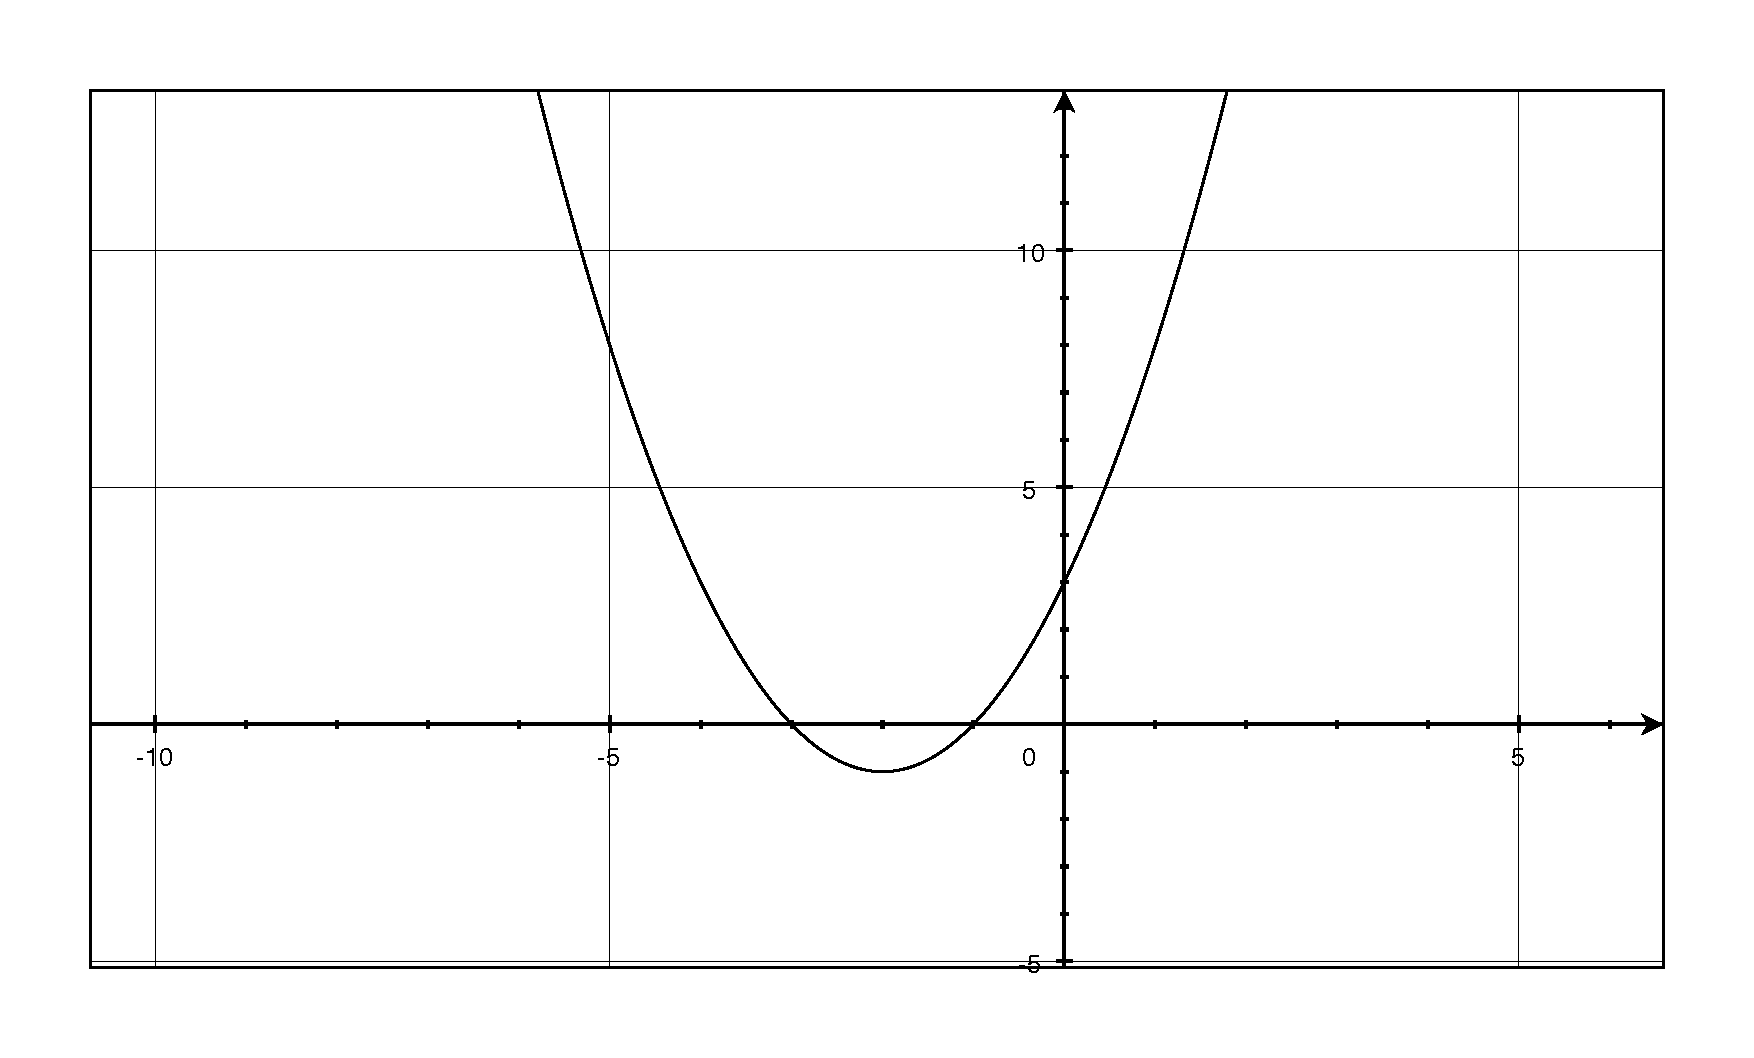
\includegraphics[scale=.3]{problem_09.eps}
        \caption*{Problem 9}
      \end{figure}

    \pagebreak

    \item[10]
      Put in standard form to find the vertex:
      \begin{align*}
        f(x) &= x^2 - 2x + 2 \\
             &= x^2 - 2x + 1 - 1 + 2 \\
             &= (x - 1)^2 + 1 \\
      \end{align*}
      The vertex is at $(1, 1)$.

      Since this parabola opens up and its vertex is at $(1, 1)$, it won't be crossing the x-axis and there won't be any
      x-intercepts.

      We can verify this by setting to 0 and trying to solve:
      \begin{align*}
          (x - 1)^2 + 1 &= 0 \\
          (x - 1)^2     &= -1 \\
          x - 1         &= \pm \sqrt{-1} \\
          x             &= 1 \pm i \\
      \end{align*}

      Find the y-intercept: $f(0) = 2$, so the y-intercept is at $(0, 2)$.

      \begin{figure}[H]
        \centering
        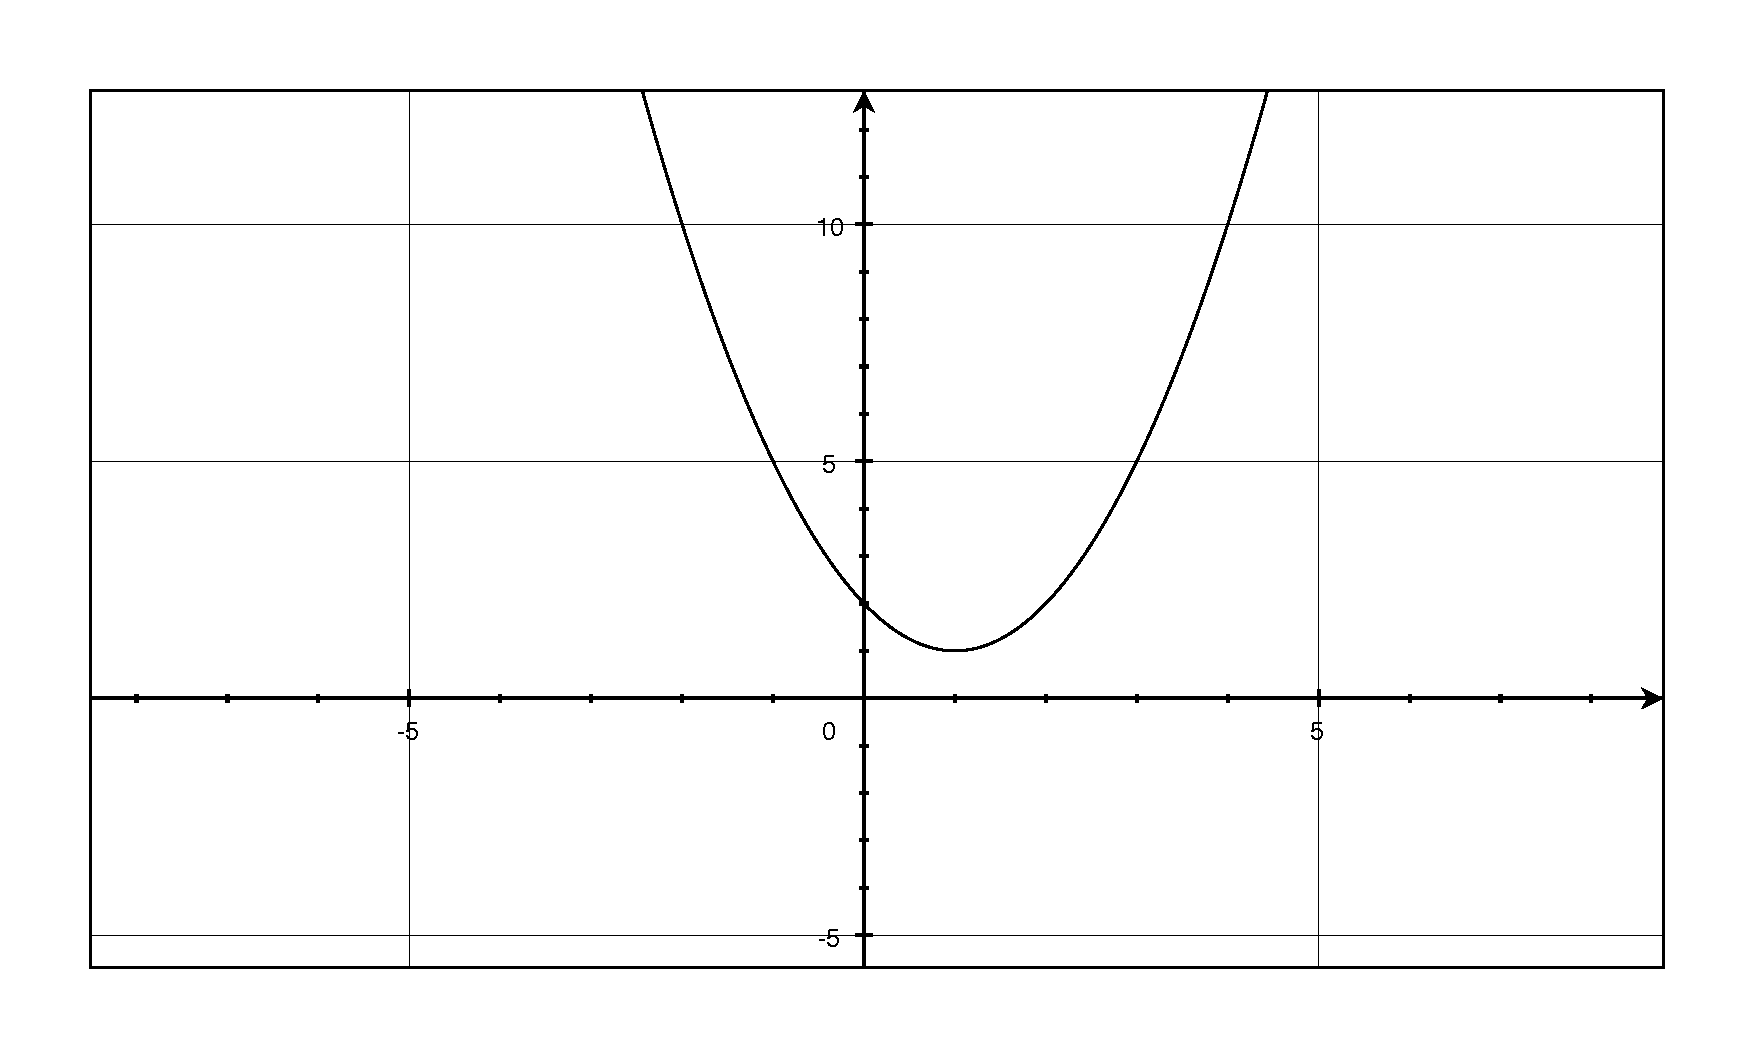
\includegraphics[scale=.3]{problem_10.eps}
        \caption*{Problem 10}
      \end{figure}

    \item[17]
      Put in standard form to find the vertex:
      \begin{align*}
        f(x) &= -4x^2 - 16x + 3 \\
             &= -4(x^2 + 4x) + 3 \\
             &= -4(x^2 + 4x + 4 - 4) + 3 \\
             &= -4(x^2 + 4x + 4) + 19 \\
             &= -4(x + 2)^2 + 19 \\
      \end{align*}
      The vertex is at $(-2, 19)$.

      Set to 0 and solve to find the x-intercepts:
      \begin{align*}
        -4(x + 2)^2 + 19 &= 0 \\
        x                &= -2 \pm \frac{\sqrt{19}}{2} \\
                         &= \left\{ -4.1794, 0.1795 \right\} \\
      \end{align*}
      The x-intercepts are at $(-4.1794, 0)$ and $(0.1795, 0)$.  

      Find the y-intercept: $f(0) = 3$, so the y-intercept is at $(0, 3)$.

      \begin{figure}[H]
        \centering
        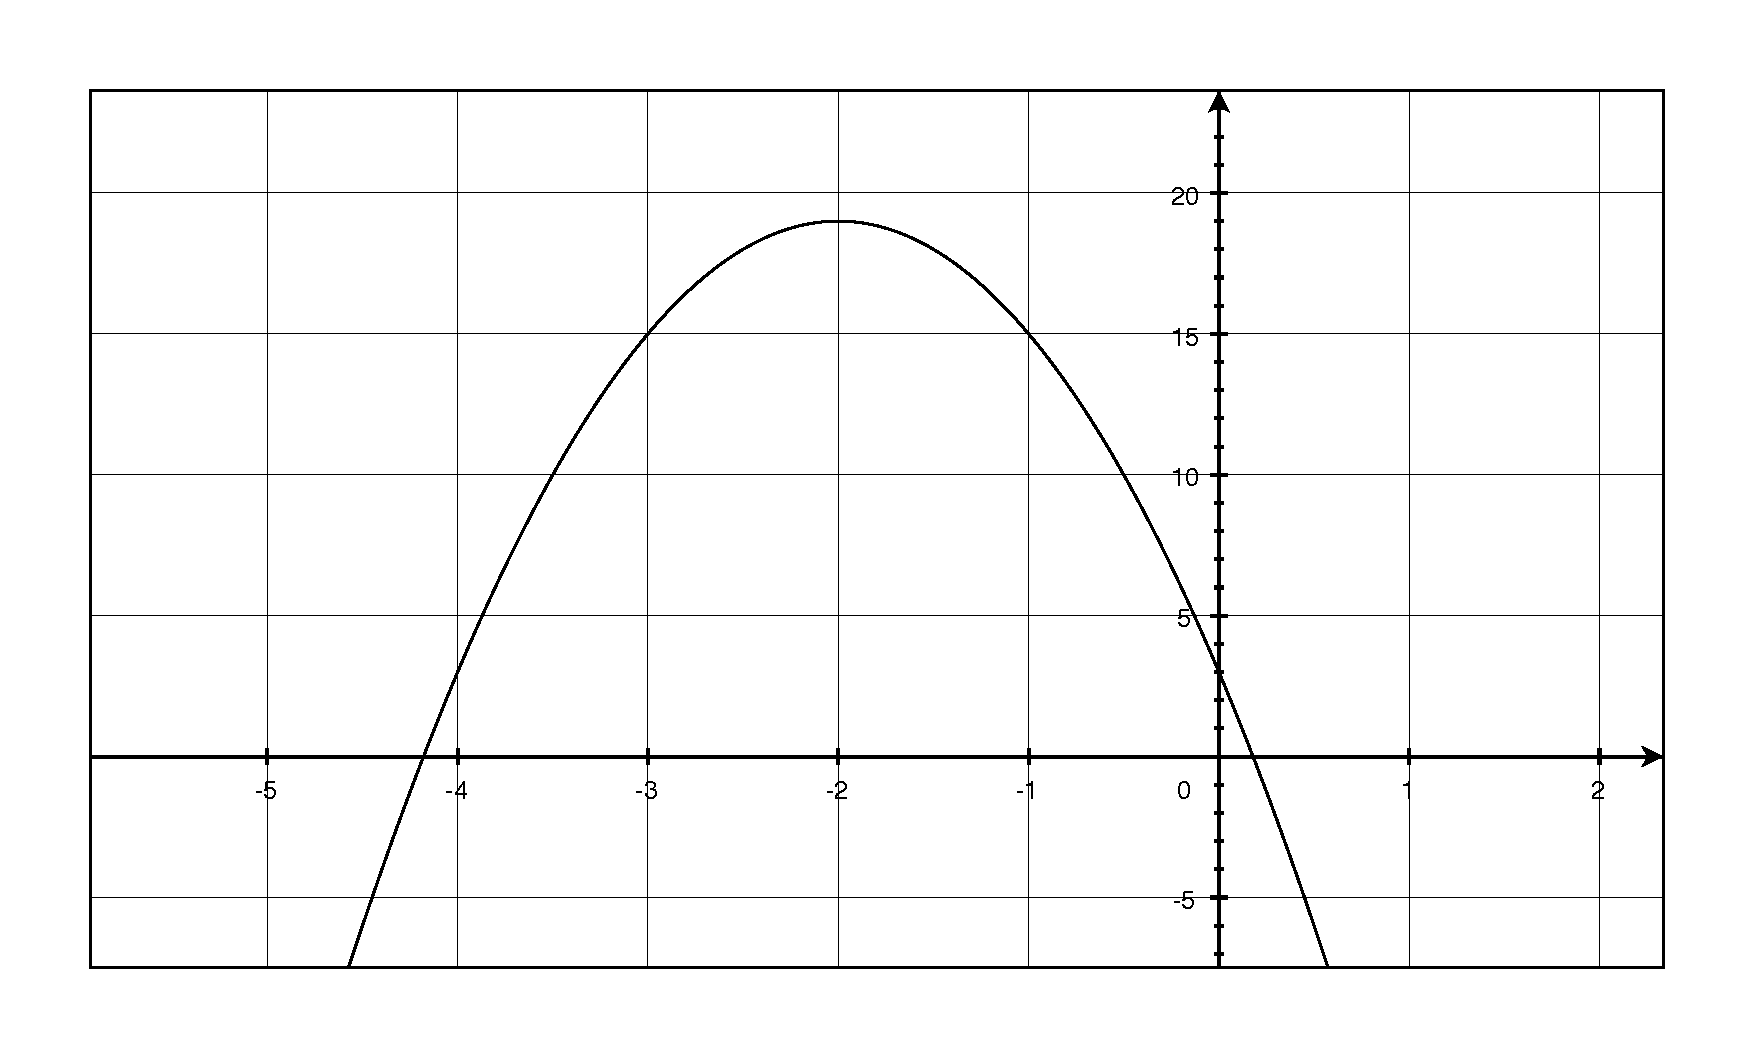
\includegraphics[scale=.3]{problem_17.eps}
        \caption*{Problem 17}
      \end{figure}

    \item[20]
      standard form:
      \begin{align*}
        f(x) &= x^2 + x \\
          &= x^2 + x + \frac{1}{4} - \frac{1}{4} \\
          &= \left(x + \frac{1}{2} \right)^2 - \frac{1}{4} \\
      \end{align*}
      The vertex/minimum is at $\left( - \frac{1}{2}, -\frac{1}{4} \right)$.

      \begin{figure}[H]
        \centering
        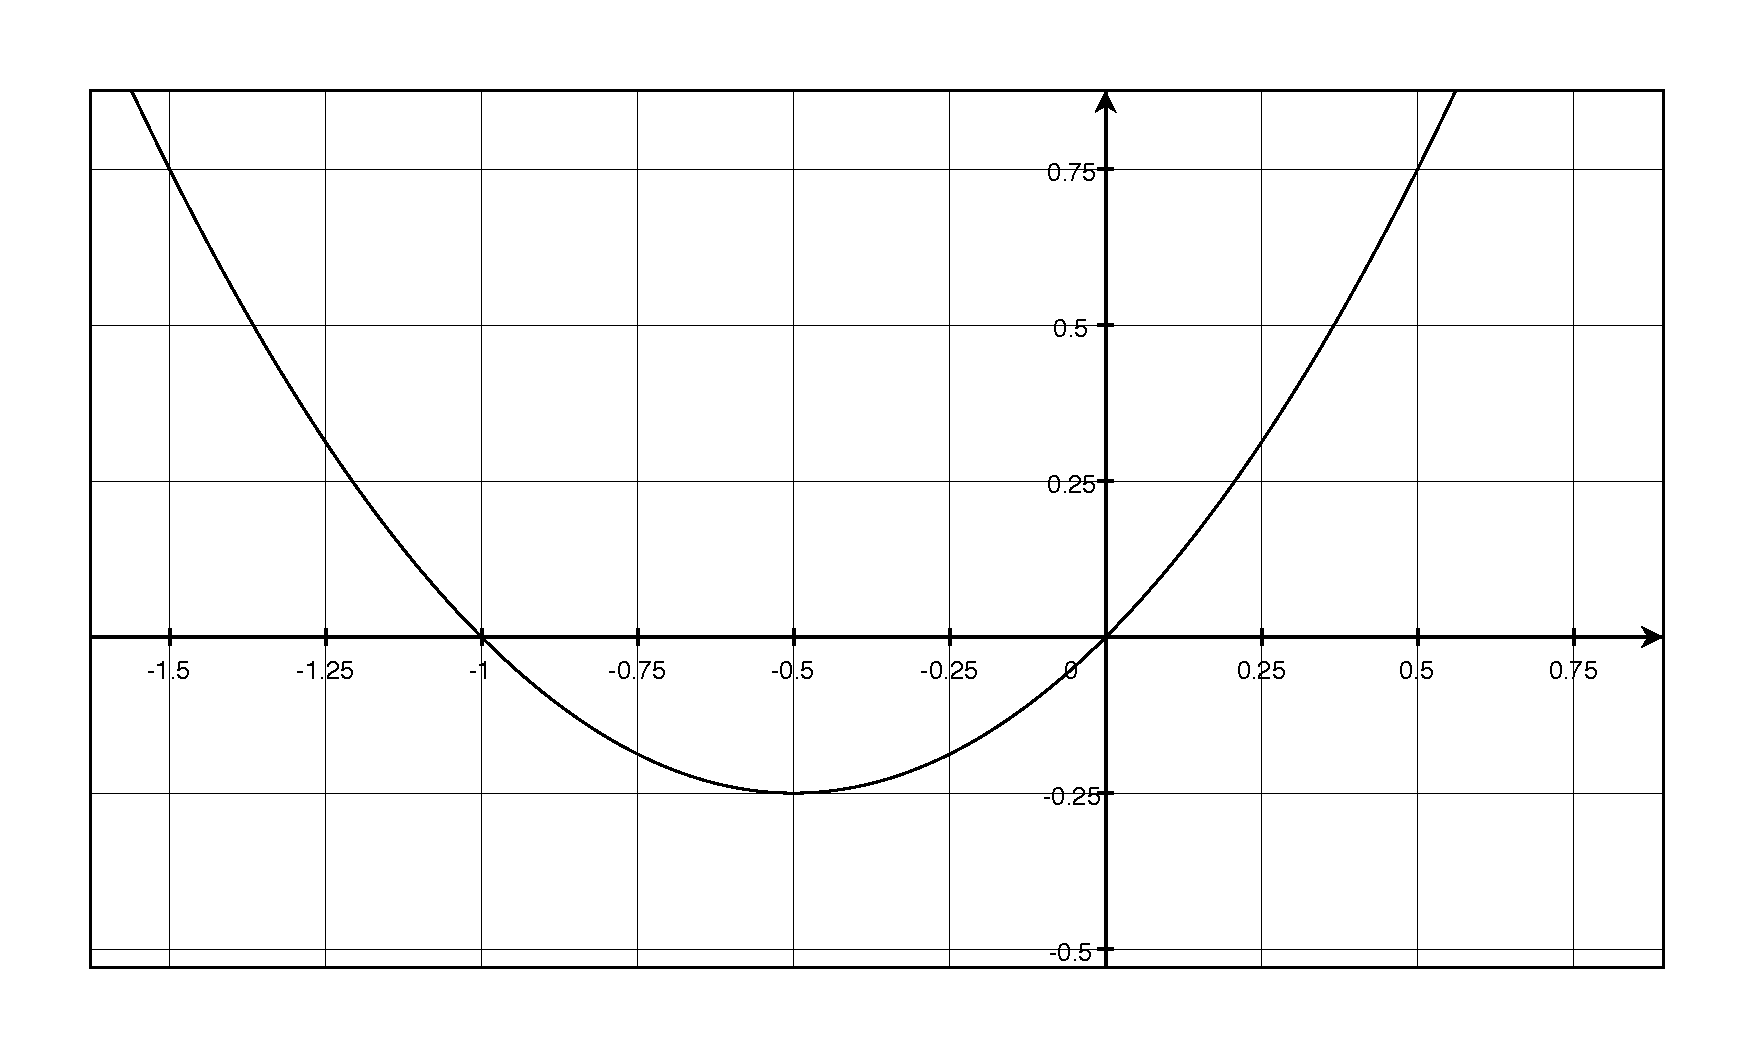
\includegraphics[scale=.3]{problem_20.eps}
        \caption*{Problem 20}
      \end{figure}

    \item[21]
      standard form:
      \begin{align*}
        f(x) &= x^2 + 2x - 1 \\
          &= x^2 + 2x + 1 - 1 - 1 \\
          &= (x + 1)^2 - 2 \\
      \end{align*}
      The vertex/minimum is at $(-1, -2)$.

      \begin{figure}[H]
        \centering
        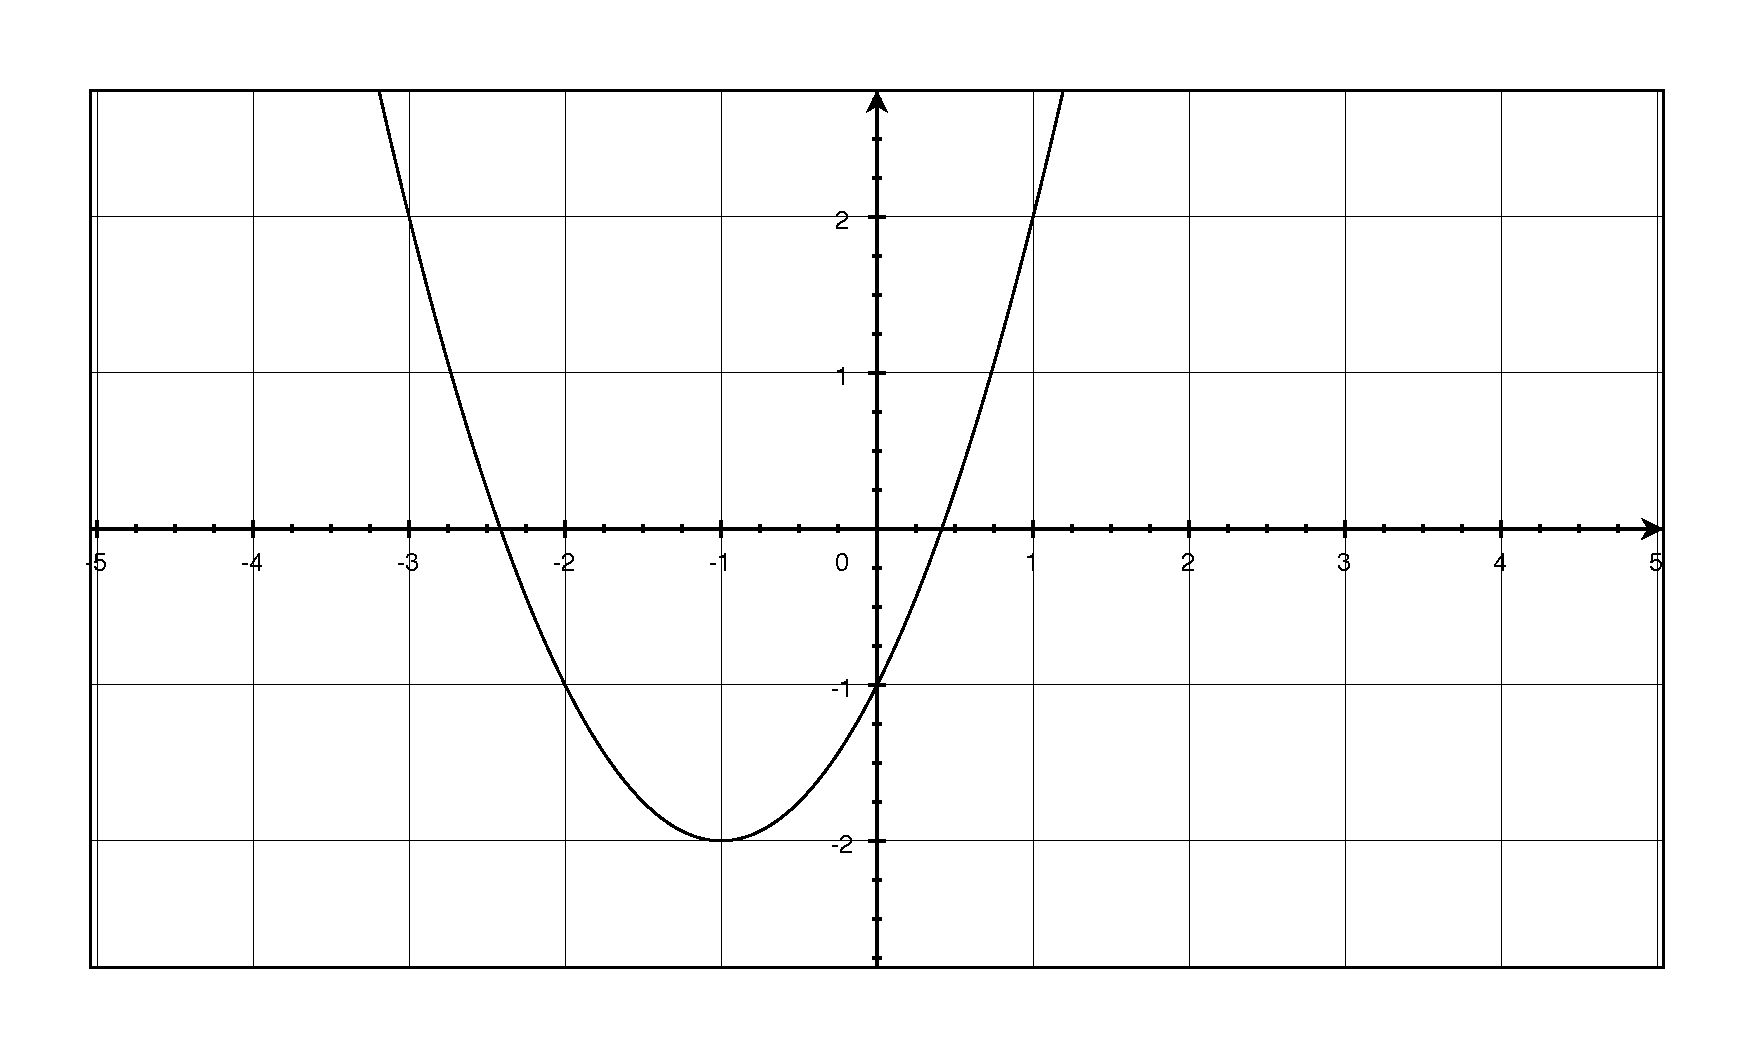
\includegraphics[scale=.3]{problem_21.eps}
        \caption*{Problem 21: $x^2 + 2x - 1$}
      \end{figure}

    \item[27]
      standard form:
      \begin{align*}
        f(x) &= 1 - x - x^2 \\
          &= -x^2 - x + 1 \\
          &= -(x^2 + x) + 1 \\
          &= -\left( x^2 + x + \frac{1}{4} - \frac{1}{4} \right) + 1 \\
          &= -\left( x^2 + x + \frac{1}{4} \right) + \frac{5}{4} \\
          &= - \left( x + \frac{1}{2} \right)^2 + \frac{5}{4} \\
      \end{align*}
      The vertex/maximum is at $\left( -\frac{1}{2}, \frac{5}{4} \right)$.

      \begin{figure}[H]
        \centering
        \includegraphics[scale=.3]{problem_27.eps}
        \caption*{Problem 27}
      \end{figure}

    \item[29]
      \begin{align*}
        x_{min}                       &= - \frac{1}{2} \\
        f\left( - \frac{1}{2} \right) &= \frac{3}{4} \\
      \end{align*}
      The minimum is at $\left( - \frac{1}{2}, \frac{3}{4} \right)$.

    \item[30]
      \begin{align*}
        x_{max}                     &= \frac{3}{2} \\
        f\left( \frac{3}{2} \right) &= \frac{13}{4} \\
      \end{align*}
      The maximum is at $\left( \frac{3}{2}, \frac{13}{4} \right)$.

    \item[35]
      \begin{align*}
        x_{min} &= \frac{-2}{2 \cdot 1/2} \\
                &= -2 \\
        f(-2)   &= -8 \\
      \end{align*}
      The minimum is at $(-2, -8)$.

    \item[38]
      standard form:
      \begin{align*}
        g(x)    &= 2x(x - 4) + 7 \\
                &= 2x^2 - 8x + 7 \\
        \\
        x_{min} &= \frac{8}{4} = 2 \\
        g(2)    &= -1 \\
      \end{align*}
      The minimum is at $(2, -1)$.

    \item[39]
      \begin{align*}
        y      &= a(x - 1)^2 - 2 \\
        16     &= a(4 - 1)^2 - 2 \\
        9a - 2 &= 16 \\
        a      &= 2 \\
      \end{align*}
      The function is: $f(x) = 2(x - 1)^2 - 2$ or $f(x) = 2x^2 - 4x$.

    \item[40]
      \begin{align*}
        y  &= a(x - 3)^2 + 4 \\
        -8 &= a(1 - 3)^2 + 4 \\
        -8 &= 4a + 4 \\
        a  &= -3 \\
      \end{align*}
      So the function is: $f(x) = -3(x - 3)^2 + 4$.  Another way to write it is $f(x) = -3x^2 + 18x - 23$.

    \item[41]
      The domain for any polynomial is $(-\infty, \infty)$.  Since the coefficient of the $x^2$ term is negative, the
      vertex is the maximum value.  Find the vertex:
      \begin{align*}
        x_{max} &= \frac{-4}{2 \cdot (-1)} = 2 \\
        f(2) &= 1 \\
      \end{align*}
      The vertex is at $(2, 1)$ and the range is $(-\infty, 1]$.

    \item[45]
      \begin{align*}
        x_{max}  &= \frac{-1.79}{2} \approx -0.8950 \\
        f(0.895) &\approx -4.011 \\
      \end{align*}

    \item[46]
      \begin{align*}
        x_{max}   &= \frac{-1}{2 \cdot (-\sqrt{2})} \approx 0.3536 \\
        f(0.3536) &\approx 1.1768 \\
      \end{align*}

    \item[47]
      \begin{itemize*}
        \item local maximum: $(0, 2)$
        \item local minimums: $(-2, -1)$ and $(2, 0)$.
      \end{itemize*}

    \item[48]
      \begin{itemize*}
        \item local maximums: $(-2, 2)$ and $(2, 1)$.
        \item local minimum: $(0, -1)$.
      \end{itemize*}

    \item[59]
      Find the vertex to find the maximum height:
      \begin{align*}
        t &= \frac{-40}{2 \cdot (-16)} = 1.25 \\
        y(1.25) &= 25 \unit{ft} \\
      \end{align*}

      The highest point reached is 25 feet.  This occurs at $t = 1.25$ seconds.

    \item[60]
      \begin{parts}
        \part To find the maximum height, we need to find the vertex:
        \begin{align*}
          x &= \frac{-1}{2 \cdot (-0.005)} = 55 \unit{ft} \\
          y(55) &= 100 \\
        \end{align*}
        The maximum height reached is 55 feet.  This happens when $x = 100$ feet.

        \part
        To find the total distance the ball traveled, we need to find the two x values which make the y coordinate is 0.
        The larger one of these is the point where the ball hits the ground at the end of the flight.  The smaller one
        is a negative number, because the ball starts out at 5 feet when was thrown by a baseball player.  The negative
        number represents the point the ball would have started if it had been launched on the same trajectory from the
        ground.

        \begin{align*}
            -0.005 (x - 100)^2 + 55 &= 0 \\
            (x - 100)^2             &= 11000 \\
            x                       &= 100 \pm \sqrt{11000} \\
                                    &= \left\{ -5, 205 \right\} \\
        \end{align*}

        The ball hits the ground at $x = 205$.

      \end{parts}

    \item[61]
      Find the vertex to find the maximum revenue:
      \begin{align*}
        x_{max} &= \frac{-80}{-2 \cdot (-0.4)} = 100 \\
        R(100)  &= 4,000 \\
      \end{align*}
      The maximum revenue of \$4,000 is achieved by making 100 units.
      
  \end{description}

  \pagebreak

  \section{Section 2.6}
  \begin{description}
    \item[1]
      If we call the length $l$ and the width $w$:
      \begin{align*}
        l    &= 3w \\
        A    &= lw \\
        \\
        A(w) &= (3w) \cdot w \\
             &= 3w^2 \\
      \end{align*}

    \item[2]
      If we call the length $l$ and the width $w$:
      \begin{align*}
        l    &= w + 10 \\
        A    &= lw \\
        \\
        A(w) &= (w + 10) \cdot w \\
             &= w^2 + 10w \\
      \end{align*}

    \item[3]
      If we call the height $h$ and the width of the base $w$:
      \begin{align*}
        h    &= \frac{w}{2} \\
        A    &= w^2h \\
        \\
        A(w) &= \frac{w^3}{2} \\
      \end{align*}

    \item[4]
      If we call the height $h$ and the radius $r$:
      \begin{align*}
        h    &= 4r \\
        V    &= \pi r^2 h \\
        \\
        V(r) &= 4 \pi r^3 \\
      \end{align*}

    \item[5] 
      If we call the sides $x$ and $y$, we can find an expression for one side in terms of the perimeter and the other
      side:
      \begin{align*}
        2x + 2y &= P \\
        x + y   &= \frac{P}{2} \\
        y       &= \frac{P}{2} - x \\
      \end{align*}

      For this problem, the perimeter is 20, so the equation for the side is $y = 10 - x$.  Now we can find the function
      for the area:
      \begin{align*}
        A    &= xy \\
        y    &= 10 - x \\
        \\
        A(x) &= x(10 - x) \\
             &= 10x - x^2 \\
      \end{align*}

    \item[12]
      There are two similar triangles, so the ratios of corresponding sides are equal:
      \begin{align*}
        \frac{L}{5} &= \frac{L + d}{12} \\
        12L         &= 5L + 5d \\
        L           &= \frac{5d}{7} \\
      \end{align*}

      So the function is: $L(d) = \frac{5d}{7}$

    \pagebreak

    \item[13]
      The functions for the two ships' positions in terms of time are:
      \begin{align*}
        x(t) &= 20t \\
        y(t) &= -15t \\
      \end{align*}

      Since they are traveling on the legs of a right triangle, the distance is:
      \begin{align*}
        d &= \sqrt{x^2 + y^2} \\
          &= \sqrt{(20t)^2 + (-15t)^2} \\
          &= \sqrt{400t^2 + 225t^2} \\
          &= 25t \\
      \end{align*}

      So the function is: $d(t) = 25t$.

    \item[17]
      If $x$ is half the length of the base:
      \begin{align*}
        x^2 + h^2 &= r^2 \\
        x         &= \sqrt{r^2 - h^2} \\
                  &= \sqrt{100 - h^2} \\
      \end{align*}

      The area of the rectangle is: $A = 2xh$.  So the function for the area in terms of the height is:
      \[
        A(h) = 2h \sqrt{100 - h^2}
      \]

    \item[20]
      \begin{align*}
        x + y &= 100 \\
        y     &= 100 - x \\
      \end{align*}

      The function is:
      \begin{align*}
        f(x) &= x^2 + y^2 \\
             &= x^2 + (100 - x)^2 \\
             &= 2x^2 - 200x + 10000 \\
      \end{align*}

      Find the minimum:
      \[
        x_{min} = \frac{200}{4} = 50 
      \]

      When $x$ is 50:
      \[
        y = 100 - x = 50 
      \]

      So the minimum occurs when $x = y = 50$.

    \item[23]
      The function for the area in terms of $x$ is:
      \begin{align*}
        A(x) &= x(2400 - 2x) \\
             &= -2x^2 + 2400x \\
      \end{align*}

      Find the maximum for $x$:
      \[
        x_{max} = \frac{-2400}{-4} = 600 \\
      \]

      So the largest area pen has dimensions 600 ft by 1200 ft which provides an area of $\SI{720,000}{ft^2}$.
  \end{description}

\else
  \vspace{9 cm}
  \begin{quote}
    \emph{All you need in life is ignorance and confidence; then success is sure.}
  \end{quote}

  \hspace{1 cm} --Mark Twain
\fi

\end{document}

